\documentclass{beamer}
\usepackage[utf8]{inputenc}
\usepackage{graphicx}
\usepackage{amsmath,amssymb}
\usepackage{mathtools}
\usepackage{amsfonts}
\usepackage{stmaryrd}
\usepackage{amsthm}
\usepackage{algorithm}
\usepackage{algpseudocode}


\usepackage{stackengine}

\usepackage{subcaption}
\usepackage[T1]{fontenc}
\usepackage{libertine}
\usepackage[scaled=0.92]{inconsolata}
\usepackage[libertine]{newtxmath}
\usepackage{tikz}
\usetikzlibrary{bayesnet}
\usepackage{adjustbox}
\usepackage{multirow, multicol}
\usepackage{caption}

\usepackage{mwe}

\usetheme{Madrid}
\usecolortheme{default}
\setbeamertemplate{navigation symbols}{}


\newcommand{\cY}{\ensuremath{\mathcal{Y}}}
\newcommand{\cR}{\ensuremath{\mathcal{R}}}
\newcommand{\cX}{\ensuremath{\mathcal{X}}}
\renewcommand{\epsilon}{\varepsilon}
\renewcommand{\phi}{\varphi}
\newcommand{\floor}[1]{\left\lfloor #1 \right\rfloor}
\newcommand{\ceil}[1]{\left\lceil #1 \right\rceil}
\newcommand{\comb}[2]{\displaystyle{#2 \choose #1}}
\newcommand{\parts}{\mathcal{P}}
\newcommand{\permut}{\mathfrak{S}}
\newcommand{\id}{\text{Id}}
\newcommand{\indic}{\mathds{1}}
\renewcommand{\leq}{\leqslant}
\renewcommand{\geq}{\geqslant}
\newcommand{\mat}[2]{\mathcal{M}_{#1}(#2)}

\newcommand{\dd}{\text{d}}
\renewcommand{\vec}{\overrightarrow}
\renewcommand{\Im}{\mathfrak{Im}\ }
\newcommand{\Ker}{\text{Ker}\ }
\newcommand{\bijective}{%
  \hookrightarrow\mathrel{\mspace{-15mu}}\rightarrow
}
\newcommand{\surjective}{\twoheadrightarrow}
\newcommand{\injective}{\hookrightarrow}
\newcommand{\implication}{\Longrightarrow}
\newcommand{\reciprocal}{\Longleftarrow}
\newcommand{\equivalent}{\Longleftrightarrow}
\newcommand{\NN}{\ensuremath{\mathbb{N}}}
\newcommand{\RR}{\ensuremath{\mathbb{R}}}
\newcommand{\QQ}{\ensuremath{\mathbb{Q}}}
\newcommand{\ZZ}{\ensuremath{\mathbb{Z}}}
\newcommand{\CC}{\ensuremath{\mathbb{C}}}
\newcommand{\EE}{\ensuremath{\mathbb{E}}}
\newcommand{\PP}{\ensuremath{\mathbb{P}}}
\newcommand{\II}{\ensuremath{\mathds{1}}}
\newcommand{\IIp}[1]{\ensuremath{\mathds{1}\left\{ #1 \right\}}}
\newcommand{\cZ}{\ensuremath{\mathcal{Z}}}
\newcommand{\cN}{\ensuremath{\mathcal{N}}}
\newcommand{\cT}{\ensuremath{\mathcal{T}}}

\DeclareMathOperator{\mut}{mut}
\DeclareMathOperator{\stab}{Stab}
\DeclareMathOperator{\sg}{sg}
\DeclareMathOperator*{\argmax}{argmax}
\DeclareMathOperator*{\argmin}{argmin}
\renewcommand{\time}{\textsc{Time}}
\newcommand{\len}{\textsc{Length}}
\newcommand{\call}[1]{\textsc{#1}}
\newcommand{\bbrack}[1]{\left\llbracket#1\right\rrbracket}

\DeclareMathOperator{\ucb}{UCB}

\author[]{Thomas \textsc{Michel}, Théo \textsc{Rudkiewicz} and Ali \textsc{Ramlaoui}}
\title[Clustering Multivariate Ordinal Data]{Clustering Multivariate Ordinal Data\\Alternative model and faster method}
\begin{document}

\frame{\titlepage}

\begin{frame}{Overview}
    \begin{itemize}
        \item Clustering multivariate ordinal data
              % \footnote{Study based on \textit{Christophe Biernacki and Julien Jacques. Model-based clustering of multivariate ordinal data relying on a stochastic binary search algorithm. Statistics and Computing, 26:929–943, 2016.}}
        \item Two univariate model: \begin{itemize}
                  \item Binary Ordinal Search (BOS)
                  \item Globally Ordered Data (GOD) $\star$
              \end{itemize}
        \item New fast parameter estimation method and open source implementation (\hyperlink{https://github.com/Thomick/Ordinal-data-clustering}{link}) $\star$
        \item New experiments $\star$
    \end{itemize}

    \hfill\small $\star$ Our contribution
\end{frame}

\begin{frame}{Univariate probabilistic models}
    $n$ samples, $m$ categories
    \begin{itemize}
        \item BOS model: Result of a binary search with noisy comparisons.
        \item GOD model: Most probable result of a linear search with noisy comparisons.
    \end{itemize}

    \begin{figure}[htbp]
        \centering
        \begin{adjustbox}{width=0.8\textwidth}
            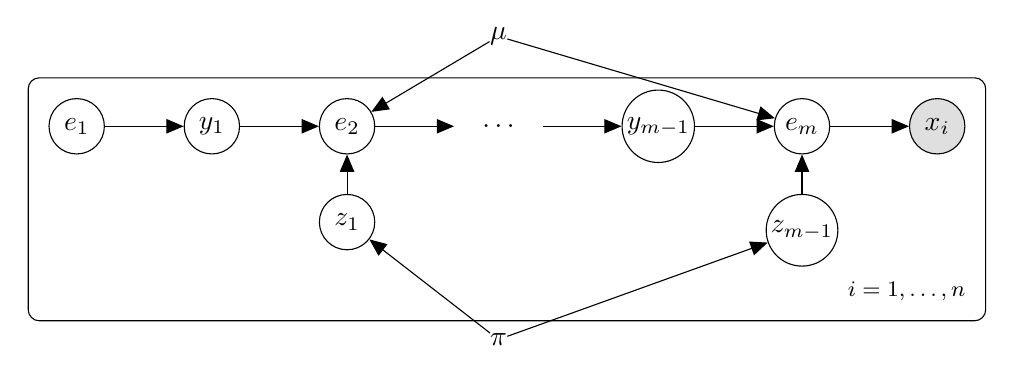
\begin{tikzpicture}
                \node[obs]                               (xi) {$x_i$};
                \node[latent, left=of xi]               (em) {$e_m$};
                \node[latent, below=of em, yshift=0.5cm]               (zm1) {$z_{m-1}$};
                \node[latent, left=of em]               (ym1) {$y_{m-1}$};
                \node[const, left=of ym1]               (dots) {$\quad\ldots\quad$};
                \node[latent, left=of dots]               (e2) {$e_2$};
                \node[latent, below=of e2, yshift=0.5cm]               (z1) {$z_1$};
                \node[latent, left=of e2]               (y1) {$y_1$};
                \node[latent, left=of y1]               (e1) {$e_1$};
                \node[const, above=of dots]    (mu) {$\mu$};
                \node[const, below=of dots, yshift=-1.6cm]  (pi) {$\pi$};

                \edge{e1}{y1};
                \edge{y1}{e2};
                \edge{z1}{e2};
                \edge{e2}{dots};
                \edge{dots}{ym1};
                \edge{ym1}{em};
                \edge{zm1}{em};
                \edge{em}{xi};
                \edge{mu}{e2};
                \edge{mu}{em};
                \edge{pi}{z1};
                \edge{pi}{zm1};

                \plate[inner sep=.25cm] {} {(xi)(e1)(zm1)(z1)} {$i=1, \ldots, n$};
            \end{tikzpicture}
        \end{adjustbox}
        \caption*{Graphical model of the stochastic Binary Ordinal Search.}
        \label{fig:graphical_model}
    \end{figure}

    \begin{figure}[htbp]
        \centering
        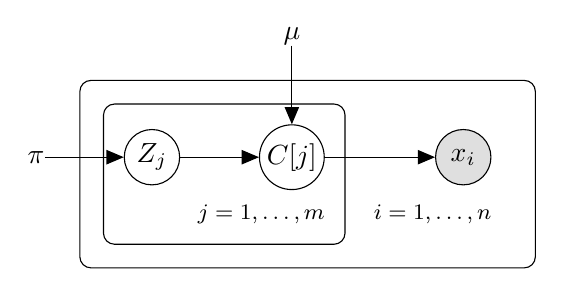
\begin{tikzpicture}
            \node[obs]                               (xj) {$x_i$};
            \node[latent, left=1.4cm of xj]               (cj) {$C[j]$};
            \node[latent, left=of cj]               (zj) {$Z_j$};
            \node[const, left=of zj]    (pi) {$\pi$};
            \node[const, above=of cj]  (mu) {$\mu$};

            \edge{zj}{cj};
            \edge{cj}{xj};
            \edge {mu} {cj};
            \edge {pi} {zj};

            \plate[inner sep=.55cm] {}{(xj)(cj)(zj)}{$i=1, \ldots, n$};
            \plate[inner sep=.25cm] {}{(cj)(zj)}{$j=1, \ldots, m$};
        \end{tikzpicture}
        \caption*{Graphical model of the GOD model.}
        \label{fig:god_graphical_model}
    \end{figure}
\end{frame}

\begin{frame}{Efficient parameter estimation}
    \begin{itemize}
        \item We show that \(\Pr(x | \mu, \pi)\) is polynomial of degree \(m - 1\) in $\pi$ with non-negative coefficients
        \item $m^2$ polynomials to compute in total. The complexity of the computation is :
              \begin{itemize}
                  \item $O(m^6)$ for the BOS model (via Lagrange interpolation)
                  \item $O(m 2^m)$ for the GOD model
              \end{itemize}
        \item Efficient computation of the log-likelihood once all the coefficients are known.
        \item Log-likelihood is concave so we can maximize it using the trisection method
        \item Final complexity for a precision of $\epsilon$:\begin{itemize}
                  \item $O(m^6)$ pre-computation then $O(n + m^3 \ln \epsilon)$ for the BOS model
                        \item$O(m2^m)$ pre-computation then $O(n + m^3 \ln \epsilon)$ for GOD model
              \end{itemize}
    \end{itemize}
\end{frame}

\begin{frame}{AECM algorithm}
    Alternating Expectation-Conditional Maximization (AECM) algorithm allows to find cluster in data where each cluster is created by the same univariate probabilistic model.

    It uses the same principle as EM but adds an estimation step of each univariate probabilistic model parameters in the maximization.
\end{frame}

\begin{frame}{Experiments}
    \begin{itemize}
        \item Test of the AECM estimation for both models on generated datasets from the corresponding distributions
    \end{itemize}

    \begin{table}[H]
        \centering
        \begin{minipage}{.48\columnwidth}
            \centering
            \begin{adjustbox}{width=\columnwidth}
                \begin{tabular}{lllllrrr}
                                                &                         &                       &                       &            & $\Delta \alpha$ & $\Delta \mu$ & $\Delta \pi$ \\
                    Init.                       & $n$                     & $n_{clusters}$        & $d$                   & $n_{cats}$ &                 &              &              \\

                    \cline{1-8} \cline{2-8} \cline{3-8} \cline{4-8}
                    \multirow[t]{16}{*}{Random} & \multirow[t]{8}{*}{250} & \multirow[t]{4}{*}{3} & \multirow[t]{2}{*}{3} & 2          & 0.095           & 0.000        & 0.035        \\
                                                &                         &                       &                       & 3          & 0.018           & 0.222        & 0.007        \\
                    \cline{4-8}
                                                &                         &                       & \multirow[t]{2}{*}{5} & 2          & 0.031           & 0.000        & 0.016        \\
                                                &                         &                       &                       & 3          & 0.017           & 0.067        & 0.019        \\
                    \cline{3-8} \cline{4-8}
                                                &                         & \multirow[t]{4}{*}{5} & \multirow[t]{2}{*}{3} & 2          & 0.037           & 0.167        & 0.022        \\
                                                &                         &                       &                       & 3          & 0.057           & 0.222        & 0.037        \\
                    \cline{4-8}
                                                &                         &                       & \multirow[t]{2}{*}{5} & 2          & 0.044           & 0.000        & 0.022        \\
                                                &                         &                       &                       & 3          & 0.020           & 0.067        & 0.052        \\
                    \cline{1-8} \cline{2-8} \cline{3-8} \cline{4-8}
                \end{tabular}
            \end{adjustbox}
            % \caption{Results of the experiments for the AECM algorithm no synthetic data with the BOS distribution. The parameters are the number of samples $n$, the number of clusters $n_{clusters}$, the dimension $d$ and the number of categories $n_{cats}$. The deltas are the average of the $L_1$ distances between the true and estimated parameters after applying optimal transport to find the correct clusters.}
            \caption*{AECM for BOS model.}
            \label{tab:results_bos}
        \end{minipage} \hspace{.02\columnwidth}%
        \begin{minipage}{.48\columnwidth}
            \centering
            \begin{adjustbox}{width=\columnwidth}
                \begin{tabular}{lllllrrr}
                                                &                         &                       &                       &            & $\Delta \alpha$ & $\Delta \mu$ & $\Delta \pi$ \\
                    Init.                       & $n$                     & $n_{clusters}$        & $d$                   & $n_{cats}$ &                 &              &              \\

                    \cline{1-8} \cline{2-8} \cline{3-8} \cline{4-8}
                    \multirow[t]{16}{*}{Random} & \multirow[t]{8}{*}{250} & \multirow[t]{4}{*}{3} & \multirow[t]{2}{*}{3} & 2          & 0.032           & 0.167        & 0.093        \\
                                                &                         &                       &                       & 3          & 0.197           & 0.222        & 0.042        \\
                    \cline{4-8}
                                                &                         &                       & \multirow[t]{2}{*}{5} & 2          & 0.014           & 0.200        & 0.050        \\
                                                &                         &                       &                       & 3          & 0.072           & 0.133        & 0.017        \\
                    \cline{3-8} \cline{4-8}
                                                &                         & \multirow[t]{4}{*}{5} & \multirow[t]{2}{*}{3} & 2          & 0.052           & 0.167        & 0.118        \\
                                                &                         &                       &                       & 3          & 0.098           & 0.889        & 0.146        \\
                    \cline{4-8}
                                                &                         &                       & \multirow[t]{2}{*}{5} & 2          & 0.058           & 0.400        & 0.085        \\
                                                &                         &                       &                       & 3          & 0.164           & 0.400        & 0.046        \\
                    \cline{1-8} \cline{2-8} \cline{3-8} \cline{4-8}
                \end{tabular}
            \end{adjustbox}
            % \caption{Results of the experiments for the AECM algorithm no synthetic data with the GOD model. The parameters are the number of samples $n$, the number of clusters $n_{clusters}$, the dimension $d$ and the number of categories $n_{cats}$. The deltas are the average of the $L_1$ distances between the true and estimated parameters after applying optimal transport to find the correct clusters.}
            \caption*{AECM for GOD model.}
            \label{tab:results_god}
        \end{minipage}
    \end{table}
\end{frame}

\begin{frame}{Experiments}

    \begin{itemize}
        \item Application of the clustering methods on real-life ordinal datasets.
    \end{itemize}
    \begin{table}
        \tiny
        \begin{adjustbox}{width=.7\columnwidth}
            \begin{tabular}{lllllll}
                                                            &                      & \textbf{Run (s)}          & \textbf{F1}               & \textbf{ARI}              \\
                Dataset                                     & Method               &                           &                           &                           \\

                \multirow[t]{6}{*}{\textbf{Zoo}}            & \textbf{BOS K-Means} & 4.75                      & 0.86                      & 0.90                      \\
                \textbf{}                                   & \textbf{GOD K-Means} & 15.12                     & \textbf{\underline{0.87}} & \textbf{\underline{0.90}} \\
                \textbf{}                                   & \textbf{K-Means}     & \textbf{\underline{0.01}} & 0.70                      & 0.58                      \\
                \textbf{}                                   & \textbf{Gaussian}    & 0.75                      & 0.79                      & 0.73                      \\
                \cline{1-5}
                \multirow[t]{6}{*}{\textbf{Car Evaluation}} & \textbf{BOS K-Means} & 415.80                    & 0.42                      & -0.01                     \\
                \textbf{}                                   & \textbf{GOD K-Means} & 19.26                     & \textbf{\underline{0.46}} & \textbf{\underline{0.05}} \\
                \textbf{}                                   & \textbf{K-Means}     & \textbf{\underline{0.01}} & 0.41                      & 0.01                      \\
                \textbf{}                                   & \textbf{Gaussian}    & 0.04                      & 0.44                      & 0.02                      \\
                \cline{1-5}
                \multirow[t]{6}{*}{\textbf{Hayes-Roth}}     & \textbf{BOS K-Means} & 101.11                    & 0.36                      & -0.01                     \\
                \textbf{}                                   & \textbf{GOD K-Means} & 8.49                      & 0.37                      & -0.01                     \\
                \textbf{}                                   & \textbf{K-Means}     & \textbf{\underline{0.00}} & 0.34                      & -0.01                     \\
                \textbf{}                                   & \textbf{Gaussian}    & 0.02                      & \textbf{\underline{0.45}} & \textbf{\underline{0.07}} \\
                \cline{1-5}
                \multirow[t]{6}{*}{\textbf{Caesarian}}      & \textbf{BOS K-Means} & 35.48                     & 0.53                      & -0.01                     \\
                \textbf{}                                   & \textbf{GOD K-Means} & 3.51                      & 0.59                      & 0.02                      \\
                \textbf{}                                   & \textbf{K-Means}     & \textbf{\underline{0.01}} & 0.56                      & 0.00                      \\
                \textbf{}                                   & \textbf{Gaussian}    & 0.02                      & \textbf{\underline{0.60}} & \textbf{\underline{0.03}} \\
                \cline{1-5}
            \end{tabular}
        \end{adjustbox}
        % \caption{
        % Results of the classification task for the different datasets and the proposed methods. 
        % The metrics are the F1-score, the accuracy, the Wasserstein distance and the adjusted rand index (ARI). 
        % The runtime is also reported. 
        % The best results for each dataset and metric are highlighted in bold and underlined. 
        % }
        \label{tab:results_real}
    \end{table}

\end{frame}


\begin{frame}{Experiments}
    Some more figure
\end{frame}

\begin{frame}{Demonstration}
    \hyperlink{https://ipolcore.ipol.im/demo/clientApp/demo.html?id=77777000487}{Open Demo (private)}
    \begin{figure}
        \includegraphics[width=0.8\textwidth]{Attachments/demo.png}
    \end{figure}
\end{frame}

\end{document}
